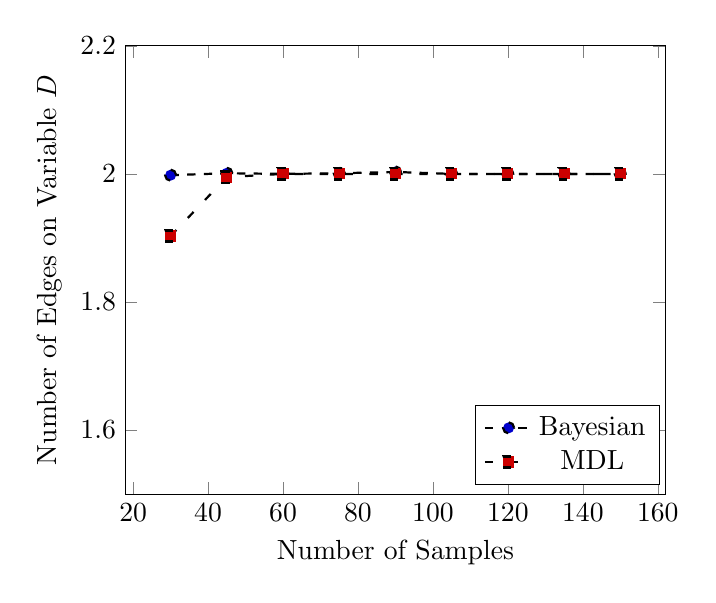
\begin{tikzpicture}
\begin{axis}[
		xlabel = Number of Samples,
		ylabel = Number of Edges on Variable $D$,
		legend style={at={(0.99,0.02)},anchor=south east},
		ymin=1.5, ymax=2.2
]
\addplot+[dashed ,black,thick] coordinates {
(30, 1.998)
(45, 2.001)
(60, 2.0)
(75, 2.001)
(90, 2.003)
(105, 2.0)
(120, 2.0)
(135, 2.0)
(150, 2.0)
};
\addlegendentry{Bayesian};

\addplot+[loosely dashed ,black,thick] coordinates {
	(30, 1.903)
	(45, 1.995)
	(60, 2.0)
	(75, 2.0)
	(90, 2.0)
	(105, 2.0)
	(120, 2.0)
	(135, 2.0)
	(150, 2.0)
};
\addlegendentry{MDL};
\end{axis}
\end{tikzpicture}
